\documentclass[letterpaper,twocolumn,10pt]{article}
\usepackage{usenix-2020-09}

\newcommand{\titlename}{
Evaluating Confidential Computing with Unikernels \\ (Guided Research Project)
}

\newcommand{\authorname}{}

\usepackage[english]{babel}
\usepackage[backend=biber]{biblatex}
\usepackage{booktabs}
\usepackage{graphicx}
\usepackage{caption}
\usepackage{subcaption}
\usepackage{tikz}
\usepackage{amsmath}
\usepackage{listings}
\usepackage{multicol}
%\usepackage{flushend}
%\usepackage[hyphens]{url}
\PassOptionsToPackage{hyphens}{url}
\usepackage{hyperref}
\hypersetup{
    colorlinks=true,
    allcolors=blue,
    breaklinks=true,
    bookmarksnumbered=true,
    bookmarkstype=toc,
    bookmarksopen=true,
    hidelinks,
    pdftitle={\titlename},
    pdfauthor={\authorname},
    pdfstartview={FitH -32768}
}

% suppress hyphenation
\hyphenpenalty=1000\relax
\exhyphenpenalty=1000\relax
\sloppy

% font
\usepackage{amsmath,amssymb,amsfonts}
\usepackage{libertine}
\usepackage{libertinust1math}
\usepackage{inconsolata}

% lsting
\usepackage{xcolor}
\definecolor{codegreen}{rgb}{0,0.6,0}
\definecolor{codegray}{rgb}{0.5,0.5,0.5}
\definecolor{codepurple}{rgb}{0.58,0,0.82}
\definecolor{backcolour}{rgb}{0.95,0.95,0.92}
\lstdefinestyle{mystyle}{
    backgroundcolor=\color{backcolour},
    commentstyle=\color{codegreen},
    keywordstyle=\color{magenta},
    numberstyle=\tiny\color{codegray},
    stringstyle=\color{codepurple},
    basicstyle=\ttfamily\footnotesize,
    breakatwhitespace=false,
    breaklines=true,
    captionpos=b,
    keepspaces=true,
    numbers=left,
    numbersep=5pt,
    showspaces=false,
    showstringspaces=false,
    showtabs=false,
    tabsize=2
}
\lstset{style=mystyle}

%\titleformat{\paragraph}[runin]{\vspace{-2pt}\bf}{}{}{\periodafter}
\newcommand{\myparagraph}{\paragraph}
\newcommand{\MP}[1]{\textcolor{red}{#1}}
\newcommand{\grumbler}[2]{\MP{{\bf #1}: #2}}
\newcommand{\note}[1]{\grumbler{NOTE}{#1}}

% bibtex
\setcounter{biburllcpenalty}{7000}
\setcounter{biburlucpenalty}{8000}
\bibliography{reference}

% watermark
\usepackage{draftwatermark}
\SetWatermarkColor[gray]{0.9}

\begin{document}

\date{}
% make title bold and 14 pt font (Latex default is non-bold, 16 pt)
\title{\Large \bf \titlename}

\author{
{\rm Roberto Castellotti}\\TU Munich
\and
{\rm Masanori Misono}\\TU Munich
}

\maketitle

\begin{abstract}
We report a preliminary performance evaluation of AMD SEV (Secure Environment Virtualization) on a Linux system.
\end{abstract}

\section{Environment}

We run our experiments on ryan, we using a patched version of QEMU from AMD.
Do we need additional info about the system?

\autoref{tab:experiment-environment} shows the detailed environment.
We use QEMU/KVM as a hypervisor.
We assign the guest the same amount of CPUs (16) and 16G of memory.

\begin{table*}[t]
\centering
\caption{Experiment environment}
\label{tab:experiment-environment}
\begin{tabular}{l|l}
\toprule
    Host CPU      & AMD EPYC 7713P 64-Cores  \\
    Host Memory   & HMAA8GR7AJR4N-XN (Hynix) 3200MHz 64 GB $\times$ 8 (512GB) \\
    Host Config   & Automatic numa balancing disabled; Side channel mitigation default (enabled) \\
    Host Kernel   & 6.1.0-rc4 \#1-NixOS SMP PREEMPT\_DYNAMIC (NixOS 22.11) \\
    QEMU          & 7.2.0 (patched) \\
\midrule
    OVMF          & Stable 202211 (patched) ????  \\
    Guest vCPU    & 16 \\
    Guest Memory  & 16GB  \\
    Guest Kernel  & 5.19.0-41-generic \#42-Ubuntu SMP PREEMPT\_DYNAMIC (Ubuntu 22.10
    ) \\
    Guest Config  & No vNUMA; Side channel mitigation default (enabled) \\
\bottomrule
\end{tabular}
\end{table*}

\section{Micro Benchmarks}

\subsection {CPU benchmarks}
We start by benchmarking the CPU by compling different programs (ffmpeg,gdb,linux kernel, llvm (ninja)) and then we ran the lz4 benchmark.

\begin{description}
    \item[compilation~\cite{compilation}] This measures how much time it takes to compile common programs. \autoref{fig:compilation} shows the results.
    \item[lz4~\cite{lz4}] We measure compression and decompression speed (MB/s). \autoref{fig:lz4-compression} and \autoref{fig:lz4-decompression}  show the results.
\end{description}


\begin{figure*}[t]
    \centering
    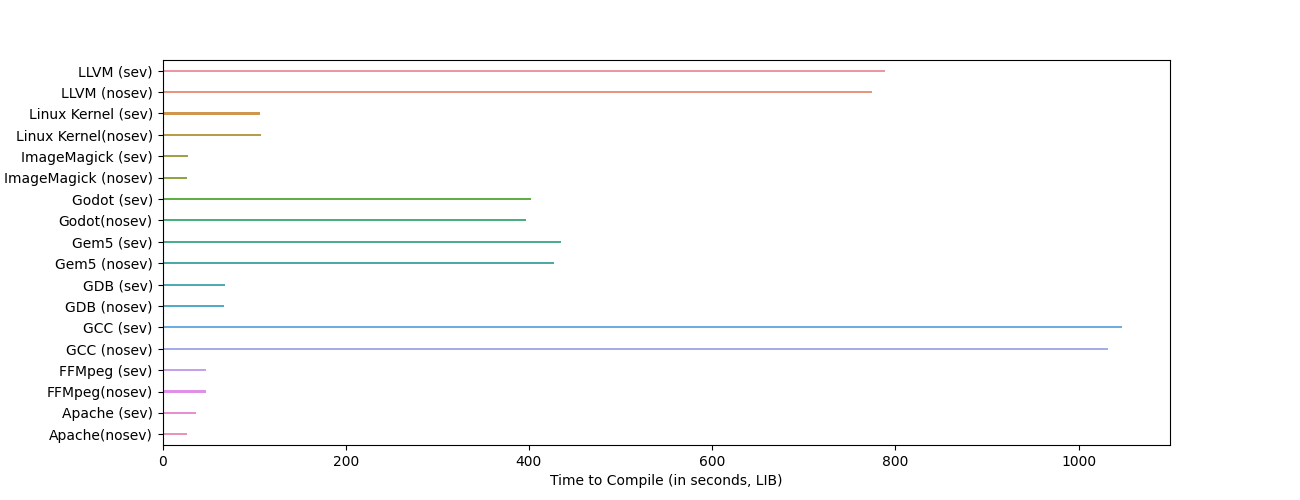
\includegraphics[width=1.0\textwidth]{../compilation.png}
    \caption{Compilation benchmark results}
    \label{fig:compilation}
\end{figure*}

\begin{figure*}[t]
    \centering
    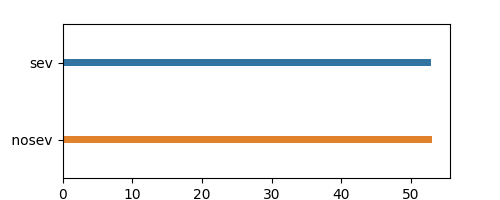
\includegraphics[width=0.5\textwidth]{../lz4-compression.png}
    \caption{LZ4 compression benchmark results}
    \label{fig:lz4-compression}
\end{figure*}

\begin{figure*}[t]
    \centering
    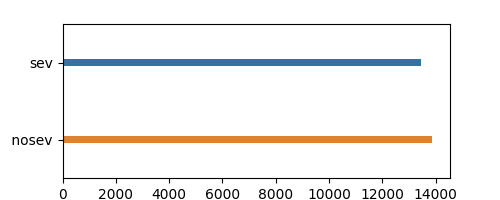
\includegraphics[width=0.5\textwidth]{../lz4-decompression.png}
    \caption{LZ4 decompression benchmark results}
    \label{fig:lz4-decompression}
\end{figure*}



\subsection{Memory overhead}
We measure the memory overhead of TDX using the following benchmarks using phoronix-test-suite~\cite{phoronix}.

\begin{description}

\item[RAMSpeed~\cite{ramspeed}] This measures the memory latency with several operations. \autoref{fig:ramspeed} shows the results.
\item[Tinymembench~\cite{tinymembench}] This benchmark measures the memory latency of the system. \autoref{fig:membench} shows the results.
\item[MBW~\cite{mbw}] This measures the memory bandwidth of the system. \autoref{fig:membench} shows the results.
\end{description}


We observe the followings from the results.
\begin{itemize}
    \item For the RAMSpeed benchmarks, we observe 3.3\% overhead for ``bare:tme'' and 6.38\% for ``vm:tdx'' in geometric mean.
    \item For the Tinymembench benchmarks, we observe 5.95\% overhead for ``bare:tme'' and 4.42\% for ``vm:tdx'' in geometric mean.
    \item For the MBW benchmarks, we observe 9.37\% overhead for ``bare:tme'' and 10.52\% for ``vm:tdx'' in geometric mean.
    \item The overhead of the memory bandwidth (MBW) is larger than the overhead of the memory latency (RAMSpeed, Tinymembench).
\end{itemize}

\section{Application Benchmarks}
\label{sec:app:benchmark}

We measure several application benchmarks using Phoronix Benchmark Suite~\cite{phoronix}.
We run and redis and SQLite benchmarks as memory-intensive applications.

\begin{description}
\item[Redis~\cite{sqlite_bench}] This measures the times of several MPI parallel applications. \autoref{fig:npb} shows the results.
\item[SQLite~\cite{sqlite_bench}] This measures the time to perform a pre-defined number of insertions to a SQLite database. \autoref{fig:membench} shows the results.
\end{description}



We observe the followings from the results.
\begin{itemize}
    \item As of compilation and NPB benchmarks, we observe around 10 to up to 60\% overhead in the TDX VM (``vm:tdx''). However, vPCU over-commitment might affect these results, so we expect the actual performance will be better.
    \item As of LZ4 benchmaks, both ``vm:notdx'' and ``vm:tdx'' have similar performance. This is because LZ4 is a memory-intensive application, and the main overhead comes from memory encryption/decryption. NPB and these results also highlight the importance of TME bypass if we want to eliminate the memory encryption overhead in non-TDX VMs.
    \item As of SQLite benchmarks, we observe larger performance overhead in ``vm:tdx'' when copy size is larger than 32. This might be due to the vCPU over-commitment, but further investigation is needed.
\end{itemize}


\printbibliography

\section*{Appendix}

\myparagraph{Check MSR values}
We can check related MSR values with the following script.
\lstinputlisting[language=c]{../sevcheck.c}

\end{document}

% this was in sevcheck.c
% // this very basic program checks whether AMD SEV features are enabled
% // we are extracting data from register 0x8000001f[EAX], as specified in 
% // paragraphs 7.10.1,15.34.1,15.35.1,15.36.1 of AMD64 Architecture Programmer’s Manual
% // amd.com/system/files/TechDocs/40332.pdf

% todo: specify what we need to check to detect what is enabled (cite the amd manual)
